\documentclass[a4paper]{book}
\usepackage{a4wide}
\usepackage{makeidx}
\usepackage{graphicx}
\usepackage{multicol}
\usepackage{float}
\usepackage{listings}
\usepackage{color}
\usepackage{textcomp}
\usepackage{alltt}
\usepackage{times}
\usepackage{ifpdf}
\ifpdf
\usepackage[pdftex,
            pagebackref=true,
            colorlinks=true,
            linkcolor=blue,
            unicode
           ]{hyperref}
\else
\usepackage[ps2pdf,
            pagebackref=true,
            colorlinks=true,
            linkcolor=blue,
            unicode
           ]{hyperref}
\usepackage{pspicture}
\fi
\usepackage[utf8]{inputenc}
\usepackage{doxygen}
\lstset{language=C++,inputencoding=utf8,basicstyle=\footnotesize,breaklines=true,breakatwhitespace=true,tabsize=8,numbers=left }
\makeindex
\setcounter{tocdepth}{3}
\renewcommand{\footrulewidth}{0.4pt}
\begin{document}
\hypersetup{pageanchor=false}
\begin{titlepage}
\vspace*{7cm}
\begin{center}
{\Large Reference Manual}\\
\vspace*{1cm}
{\large Generated by Doxygen 1.6.1}\\
\vspace*{0.5cm}
{\small Tue Dec 9 13:23:35 2014}\\
\end{center}
\end{titlepage}
\clearemptydoublepage
\pagenumbering{roman}
\tableofcontents
\clearemptydoublepage
\pagenumbering{arabic}
\hypersetup{pageanchor=true}
\chapter{Class Index}
\section{Class Hierarchy}
This inheritance list is sorted roughly, but not completely, alphabetically\-:\begin{DoxyCompactList}
\item \contentsline{section}{card}{\pageref{structcard}}{}
\item \contentsline{section}{G\-U\-I\-:\-:Card\-Info}{\pageref{structGUI_1_1CardInfo}}{}
\item \contentsline{section}{comms}{\pageref{classcomms}}{}
\item \contentsline{section}{data}{\pageref{structdata}}{}
\item \contentsline{section}{G\-U\-I\-:\-:Dealer\-G\-U\-I}{\pageref{classGUI_1_1DealerGUI}}{}
\item \contentsline{section}{dealer\-Lib}{\pageref{classdealerLib}}{}
\item \contentsline{section}{deck}{\pageref{classdeck}}{}
\item \contentsline{section}{display}{\pageref{classdisplay}}{}
\item \contentsline{section}{G\-U\-I\-:\-:Element}{\pageref{classGUI_1_1Element}}{}
\begin{DoxyCompactList}
\item \contentsline{section}{G\-U\-I\-:\-:Card}{\pageref{classGUI_1_1Card}}{}
\item \contentsline{section}{G\-U\-I\-:\-:Label}{\pageref{classGUI_1_1Label}}{}
\end{DoxyCompactList}
\item \contentsline{section}{G\-U\-I\-:\-:Element\-Maker}{\pageref{classGUI_1_1ElementMaker}}{}
\item \contentsline{section}{G\-U\-I\-:\-:Hand}{\pageref{classGUI_1_1Hand}}{}
\item \contentsline{section}{input}{\pageref{classinput}}{}
\item \contentsline{section}{G\-U\-I\-:\-:Label\-Format}{\pageref{structGUI_1_1LabelFormat}}{}
\item \contentsline{section}{G\-U\-I\-:\-:Player}{\pageref{structGUI_1_1Player}}{}
\item \contentsline{section}{player}{\pageref{classplayer}}{}
\item \contentsline{section}{Playing\-Card}{\pageref{classPlayingCard}}{}
\item \contentsline{section}{Comms\-:\-:Serial\-Port}{\pageref{classComms_1_1SerialPort}}{}
\item vector\begin{DoxyCompactList}
\item \contentsline{section}{card\-Stack}{\pageref{classcardStack}}{}
\end{DoxyCompactList}
\end{DoxyCompactList}

\chapter{Class Index}
\section{Class List}
Here are the classes, structs, unions and interfaces with brief descriptions\-:\begin{DoxyCompactList}
\item\contentsline{section}{\hyperlink{classGUI_1_1Card}{G\-U\-I\-::\-Card} \\*A visual representation of a playing card that can be flipped, burned and moved around }{\pageref{classGUI_1_1Card}}{}
\item\contentsline{section}{\hyperlink{structcard}{card} }{\pageref{structcard}}{}
\item\contentsline{section}{\hyperlink{structGUI_1_1CardInfo}{G\-U\-I\-::\-Card\-Info} \\*This struct contains variables for S\-D\-L that will be the same for all cards, which we therefore won't want to send to the constructor individually every time }{\pageref{structGUI_1_1CardInfo}}{}
\item\contentsline{section}{\hyperlink{classcardStack}{card\-Stack} }{\pageref{classcardStack}}{}
\item\contentsline{section}{\hyperlink{classcomms}{comms} }{\pageref{classcomms}}{}
\item\contentsline{section}{\hyperlink{structdata}{data} \\*Comms.\-h }{\pageref{structdata}}{}
\item\contentsline{section}{\hyperlink{classGUI_1_1DealerGUI}{G\-U\-I\-::\-Dealer\-G\-U\-I} \\*The main class used for displaying things on the screen }{\pageref{classGUI_1_1DealerGUI}}{}
\item\contentsline{section}{\hyperlink{classdealerLib}{dealer\-Lib} }{\pageref{classdealerLib}}{}
\item\contentsline{section}{\hyperlink{classdeck}{deck} }{\pageref{classdeck}}{}
\item\contentsline{section}{\hyperlink{classdisplay}{display} }{\pageref{classdisplay}}{}
\item\contentsline{section}{\hyperlink{classGUI_1_1Element}{G\-U\-I\-::\-Element} \\*The base class for any visual elements on the screen }{\pageref{classGUI_1_1Element}}{}
\item\contentsline{section}{\hyperlink{classGUI_1_1ElementMaker}{G\-U\-I\-::\-Element\-Maker} \\*This class serves as a factory for dynamically allocated visual elements }{\pageref{classGUI_1_1ElementMaker}}{}
\item\contentsline{section}{\hyperlink{classGUI_1_1Hand}{G\-U\-I\-::\-Hand} \\*This class is simply for easy manipulation of a number of cards at once. Despite the name, it does not necessarily refer to the cards a player is holding }{\pageref{classGUI_1_1Hand}}{}
\item\contentsline{section}{\hyperlink{classinput}{input} \\*Input class }{\pageref{classinput}}{}
\item\contentsline{section}{\hyperlink{classGUI_1_1Label}{G\-U\-I\-::\-Label} \\*A simple line of text constructed using S\-D\-L's T\-T\-F library that can be moved around as with other visual elements }{\pageref{classGUI_1_1Label}}{}
\item\contentsline{section}{\hyperlink{structGUI_1_1LabelFormat}{G\-U\-I\-::\-Label\-Format} \\*This struct contains variables for S\-D\-L that will be the same for all labels, which we therefore won't want to send to the constructor individually every time }{\pageref{structGUI_1_1LabelFormat}}{}
\item\contentsline{section}{\hyperlink{structGUI_1_1Player}{G\-U\-I\-::\-Player} \\*Since the \hyperlink{namespaceGUI}{G\-U\-I} requires a little more information about a given player than is contained in the player class, this struct contains that information as well as a pointer to the original class }{\pageref{structGUI_1_1Player}}{}
\item\contentsline{section}{\hyperlink{classplayer}{player} \\*Player class }{\pageref{classplayer}}{}
\item\contentsline{section}{\hyperlink{classPlayingCard}{Playing\-Card} \\*The \hyperlink{classPlayingCard}{Playing\-Card} class The \hyperlink{classPlayingCard}{Playing\-Card} class encapsulates the single byte card representation defined in \char`\"{}card.\-h\char`\"{}. It overloads various operators for ease of playing card comparison and provides string lookup tables for string representations of the card }{\pageref{classPlayingCard}}{}
\item\contentsline{section}{\hyperlink{classComms_1_1SerialPort}{Comms\-::\-Serial\-Port} \\*Encapsulates sending and recieving data from a player. It assumes the protocol is to open a transmission by sending a header byte containing both the type (left nibble) and the size of the byte payload (right nibble), any bytes sent after the header are considered the payload }{\pageref{classComms_1_1SerialPort}}{}
\end{DoxyCompactList}

\chapter{File Index}
\section{File List}
Here is a list of all files with brief descriptions\-:\begin{DoxyCompactList}
\item\contentsline{section}{include/\hyperlink{include_2comms_8h}{comms.\-h} }{\pageref{include_2comms_8h}}{}
\item\contentsline{section}{include/comms/\hyperlink{Dealer_8h}{Dealer.\-h} }{\pageref{Dealer_8h}}{}
\item\contentsline{section}{include/comms/\hyperlink{dealerIO_8h}{dealer\-I\-O.\-h} \\*An interface for the Dealer team to communicate with the Arduino players, provides utility functions for all the data that needs to be sent/recieved }{\pageref{dealerIO_8h}}{}
\item\contentsline{section}{include/comms/\hyperlink{SerialPort_8h}{Serial\-Port.\-h} \\*Encapsulates writing/reading data to/from an Arduino over the serial port }{\pageref{SerialPort_8h}}{}
\item\contentsline{section}{include/dealer/\hyperlink{cardStack_8h}{card\-Stack.\-h} }{\pageref{cardStack_8h}}{}
\item\contentsline{section}{include/dealer/\hyperlink{include_2dealer_2comms_8h}{comms.\-h} }{\pageref{include_2dealer_2comms_8h}}{}
\item\contentsline{section}{include/dealer/\hyperlink{dealerLib_8h}{dealer\-Lib.\-h} }{\pageref{dealerLib_8h}}{}
\item\contentsline{section}{include/dealer/\hyperlink{deck_8h}{deck.\-h} }{\pageref{deck_8h}}{}
\item\contentsline{section}{include/dealer/\hyperlink{include_2dealer_2player_8h}{player.\-h} }{\pageref{include_2dealer_2player_8h}}{}
\item\contentsline{section}{include/dealer/\hyperlink{playingcard_8h}{playingcard.\-h} \\*Encapsulates the low-\/level byte sized card defined in card.\-h in a user friendly class. Provides lookup functions for easy printing and comparison functions }{\pageref{playingcard_8h}}{}
\item\contentsline{section}{include/dealer/\hyperlink{pokerHands_8h}{poker\-Hands.\-h} }{\pageref{pokerHands_8h}}{}
\item\contentsline{section}{include/gui/\hyperlink{gui__card_8h}{gui\-\_\-card.\-h} }{\pageref{gui__card_8h}}{}
\item\contentsline{section}{include/gui/\hyperlink{gui__dealergui_8h}{gui\-\_\-dealergui.\-h} }{\pageref{gui__dealergui_8h}}{}
\item\contentsline{section}{include/gui/\hyperlink{gui__element_8h}{gui\-\_\-element.\-h} }{\pageref{gui__element_8h}}{}
\item\contentsline{section}{include/gui/\hyperlink{gui__elementmaker_8h}{gui\-\_\-elementmaker.\-h} }{\pageref{gui__elementmaker_8h}}{}
\item\contentsline{section}{include/gui/\hyperlink{gui__hand_8h}{gui\-\_\-hand.\-h} }{\pageref{gui__hand_8h}}{}
\item\contentsline{section}{include/gui/\hyperlink{gui__label_8h}{gui\-\_\-label.\-h} }{\pageref{gui__label_8h}}{}
\item\contentsline{section}{include/player/\hyperlink{EchoSerialInput_8h}{Echo\-Serial\-Input.\-h} }{\pageref{EchoSerialInput_8h}}{}
\item\contentsline{section}{include/shared/\hyperlink{include_2shared_2card_8h}{card.\-h} }{\pageref{include_2shared_2card_8h}}{}
\item\contentsline{section}{src/comms/\hyperlink{comms__main_8cpp}{comms\-\_\-main.\-cpp} }{\pageref{comms__main_8cpp}}{}
\item\contentsline{section}{src/comms/\hyperlink{dealerIO_8cpp}{dealer\-I\-O.\-cpp} }{\pageref{dealerIO_8cpp}}{}
\item\contentsline{section}{src/comms/\hyperlink{SerialPort_8cpp}{Serial\-Port.\-cpp} }{\pageref{SerialPort_8cpp}}{}
\item\contentsline{section}{src/dealer/\hyperlink{cardStack_8cpp}{card\-Stack.\-cpp} }{\pageref{cardStack_8cpp}}{}
\item\contentsline{section}{src/dealer/\hyperlink{comms_8cpp}{comms.\-cpp} }{\pageref{comms_8cpp}}{}
\item\contentsline{section}{src/dealer/\hyperlink{dealer__main_8cpp}{dealer\-\_\-main.\-cpp} }{\pageref{dealer__main_8cpp}}{}
\item\contentsline{section}{src/dealer/\hyperlink{dealerLib_8cpp}{dealer\-Lib.\-cpp} }{\pageref{dealerLib_8cpp}}{}
\item\contentsline{section}{src/dealer/\hyperlink{dealerLibMain_8cpp}{dealer\-Lib\-Main.\-cpp} }{\pageref{dealerLibMain_8cpp}}{}
\item\contentsline{section}{src/dealer/\hyperlink{deck_8cpp}{deck.\-cpp} }{\pageref{deck_8cpp}}{}
\item\contentsline{section}{src/dealer/\hyperlink{dealer_2player_8cpp}{player.\-cpp} }{\pageref{dealer_2player_8cpp}}{}
\item\contentsline{section}{src/dealer/\hyperlink{playingcard_8cpp}{playingcard.\-cpp} }{\pageref{playingcard_8cpp}}{}
\item\contentsline{section}{src/dealer/\hyperlink{pokerHands_8cpp}{poker\-Hands.\-cpp} }{\pageref{pokerHands_8cpp}}{}
\item\contentsline{section}{src/gui/\hyperlink{gui__card_8cpp}{gui\-\_\-card.\-cpp} }{\pageref{gui__card_8cpp}}{}
\item\contentsline{section}{src/gui/\hyperlink{gui__dealergui_8cpp}{gui\-\_\-dealergui.\-cpp} }{\pageref{gui__dealergui_8cpp}}{}
\item\contentsline{section}{src/gui/\hyperlink{gui__element_8cpp}{gui\-\_\-element.\-cpp} }{\pageref{gui__element_8cpp}}{}
\item\contentsline{section}{src/gui/\hyperlink{gui__elementmaker_8cpp}{gui\-\_\-elementmaker.\-cpp} }{\pageref{gui__elementmaker_8cpp}}{}
\item\contentsline{section}{src/gui/\hyperlink{gui__hand_8cpp}{gui\-\_\-hand.\-cpp} }{\pageref{gui__hand_8cpp}}{}
\item\contentsline{section}{src/gui/\hyperlink{gui__label_8cpp}{gui\-\_\-label.\-cpp} }{\pageref{gui__label_8cpp}}{}
\item\contentsline{section}{src/gui/\hyperlink{gui__mainExample_8cpp}{gui\-\_\-main\-Example.\-cpp} }{\pageref{gui__mainExample_8cpp}}{}
\item\contentsline{section}{src/player/\-Main\-Sketch/\hyperlink{src_2player_2MainSketch_2card_8h}{card.\-h} }{\pageref{src_2player_2MainSketch_2card_8h}}{}
\item\contentsline{section}{src/player/\-Main\-Sketch/\hyperlink{src_2player_2MainSketch_2comms_8h}{comms.\-h} }{\pageref{src_2player_2MainSketch_2comms_8h}}{}
\item\contentsline{section}{src/player/\-Main\-Sketch/\hyperlink{MainSketch_2input_8cpp}{input.\-cpp} }{\pageref{MainSketch_2input_8cpp}}{}
\item\contentsline{section}{src/player/\-Main\-Sketch/\hyperlink{MainSketch_2input_8h}{input.\-h} }{\pageref{MainSketch_2input_8h}}{}
\item\contentsline{section}{src/player/\-Main\-Sketch/\hyperlink{player_2MainSketch_2player_8cpp}{player.\-cpp} }{\pageref{player_2MainSketch_2player_8cpp}}{}
\item\contentsline{section}{src/player/\-Main\-Sketch/\hyperlink{src_2player_2MainSketch_2player_8h}{player.\-h} }{\pageref{src_2player_2MainSketch_2player_8h}}{}
\item\contentsline{section}{src/player/\-Main\-Sketch/\hyperlink{MainSketch_2pokerDisplay_8cpp}{poker\-Display.\-cpp} }{\pageref{MainSketch_2pokerDisplay_8cpp}}{}
\item\contentsline{section}{src/player/\-Main\-Sketch/\hyperlink{MainSketch_2pokerDisplay_8h}{poker\-Display.\-h} }{\pageref{MainSketch_2pokerDisplay_8h}}{}
\item\contentsline{section}{src/player/old/display/\hyperlink{old_2display_2pokerDisplay_8cpp}{poker\-Display.\-cpp} }{\pageref{old_2display_2pokerDisplay_8cpp}}{}
\item\contentsline{section}{src/player/old/display/\hyperlink{old_2display_2pokerDisplay_8h}{poker\-Display.\-h} }{\pageref{old_2display_2pokerDisplay_8h}}{}
\item\contentsline{section}{src/player/old/input/\hyperlink{old_2input_2input_8cpp}{input.\-cpp} }{\pageref{old_2input_2input_8cpp}}{}
\item\contentsline{section}{src/player/old/input/\hyperlink{old_2input_2input_8h}{input.\-h} }{\pageref{old_2input_2input_8h}}{}
\item\contentsline{section}{src/player/old/player/\hyperlink{player_2old_2player_2player_8cpp}{player.\-cpp} }{\pageref{player_2old_2player_2player_8cpp}}{}
\item\contentsline{section}{src/player/old/player/\hyperlink{src_2player_2old_2player_2player_8h}{player.\-h} }{\pageref{src_2player_2old_2player_2player_8h}}{}
\end{DoxyCompactList}

\chapter{Class Documentation}
\input{classCard}
\include{structCardInfo}
\include{classDealerGUI}
\include{classElement}
\include{classLabel}
\include{structLabelFormat}
\include{classListMenu}
\include{classTestElement}
\chapter{File Documentation}
\hypertarget{fuck_8cpp}{
\section{fuck.cpp File Reference}
\label{fuck_8cpp}\index{fuck.cpp@{fuck.cpp}}
}
{\ttfamily \#include $<$SDL2/SDL.h$>$}\par
{\ttfamily \#include $<$SDL2/SDL\_\-ttf.h$>$}\par
{\ttfamily \#include $<$cstdlib$>$}\par
{\ttfamily \#include $<$iostream$>$}\par
Include dependency graph for fuck.cpp:\nopagebreak
\begin{figure}[H]
\begin{center}
\leavevmode
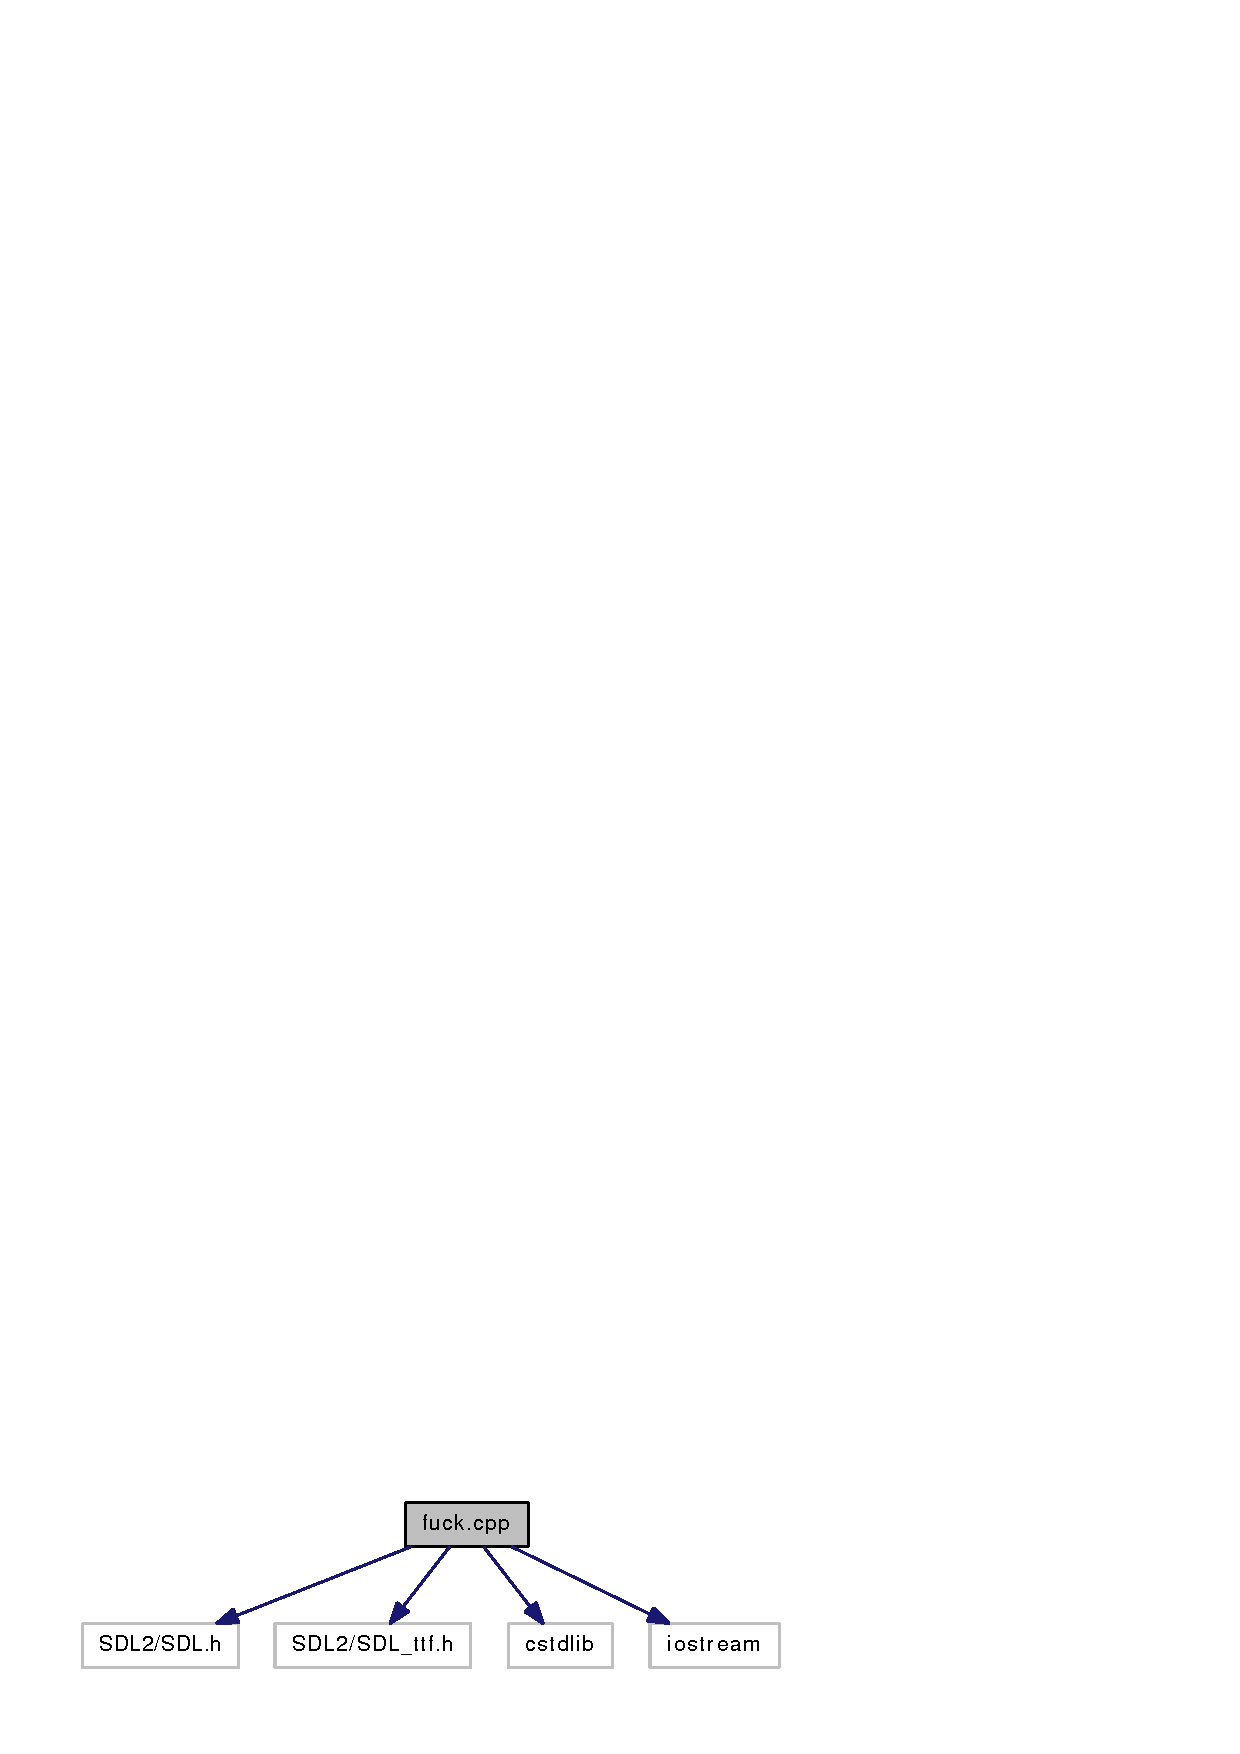
\includegraphics[width=189pt]{fuck_8cpp__incl}
\end{center}
\end{figure}
\subsection*{Functions}
\begin{DoxyCompactItemize}
\item 
int \hyperlink{fuck_8cpp_a3c04138a5bfe5d72780bb7e82a18e627}{main} (int argc, char $\ast$$\ast$argv)
\end{DoxyCompactItemize}
\subsection*{Variables}
\begin{DoxyCompactItemize}
\item 
const int \hyperlink{fuck_8cpp_a5e6ce0dd58078611570510dc4b8d81f3}{WINDOW\_\-WIDTH} = 1024
\item 
const int \hyperlink{fuck_8cpp_ab76d138fa589df9a65fc05eb3bd56073}{WINDOW\_\-HEIGHT} = 720
\end{DoxyCompactItemize}


\subsection{Function Documentation}
\hypertarget{fuck_8cpp_a3c04138a5bfe5d72780bb7e82a18e627}{
\index{fuck.cpp@{fuck.cpp}!main@{main}}
\index{main@{main}!fuck.cpp@{fuck.cpp}}
\subsubsection[{main}]{\setlength{\rightskip}{0pt plus 5cm}int main (int {\em argc}, \/  char $\ast$$\ast$ {\em argv})}}
\label{fuck_8cpp_a3c04138a5bfe5d72780bb7e82a18e627}


\subsection{Variable Documentation}
\hypertarget{fuck_8cpp_ab76d138fa589df9a65fc05eb3bd56073}{
\index{fuck.cpp@{fuck.cpp}!WINDOW\_\-HEIGHT@{WINDOW\_\-HEIGHT}}
\index{WINDOW\_\-HEIGHT@{WINDOW\_\-HEIGHT}!fuck.cpp@{fuck.cpp}}
\subsubsection[{WINDOW\_\-HEIGHT}]{\setlength{\rightskip}{0pt plus 5cm}const int {\bf WINDOW\_\-HEIGHT} = 720}}
\label{fuck_8cpp_ab76d138fa589df9a65fc05eb3bd56073}
\hypertarget{fuck_8cpp_a5e6ce0dd58078611570510dc4b8d81f3}{
\index{fuck.cpp@{fuck.cpp}!WINDOW\_\-WIDTH@{WINDOW\_\-WIDTH}}
\index{WINDOW\_\-WIDTH@{WINDOW\_\-WIDTH}!fuck.cpp@{fuck.cpp}}
\subsubsection[{WINDOW\_\-WIDTH}]{\setlength{\rightskip}{0pt plus 5cm}const int {\bf WINDOW\_\-WIDTH} = 1024}}
\label{fuck_8cpp_a5e6ce0dd58078611570510dc4b8d81f3}

\include{card_8h}
\include{dealergui_8h}
\include{element_8h}
\include{label_8h}
\include{listmenu_8h}
\include{testelement_8h}
\include{card_8cpp}
\include{dealergui_8cpp}
\include{element_8cpp}
\include{label_8cpp}
\include{listmenu_8cpp}
\include{main_8cpp}
\include{testelement_8cpp}
\printindex
\end{document}
